\chapter{Implementierung}\label{ch:impl}

\section{Spieler Steuerung}\label{sec:4_SpielerSteuerung}

Die Spieler Steuerung wird mithilfe eines Observer Patterns realisiert. Beim Laden der \josieclass{BossPlayer} Klasse wird der Spieler als Observer eingetragen:

\begin{lstlisting}[label=lst:player_control_observer,
				   language=C++,
				   firstnumber=103,
				   caption=BossPlayer als Observer eintragen ( BossPlayer.cpp )]
EventDispatcher *ed = Director::getInstance()->getEventDispatcher();
if (reg) {
	ed->addCustomEventListener("BOSS_PLAYER_LEFT", CC_CALLBACK_0(BossPlayer::moveLeft, this));
\end{lstlisting}

Die Methode \textbf{addCustomEventListener()} erwartet zwei Parameter. Den Namen auf den der Observer hören soll, und das Callback, also die Funktion die ausgeführt werden soll beim Eintreffen einer solchen Nachricht, in diesem Fall \textbf{moveLeft()}. 
Gleichbedeutend muss der Spieler auch wieder aus der Liste der Observer entfernt werden, sobald die Instanz gelöscht wird. Beides passiert über dieselbe Methode, die mit dem Parameter \textbf{false} die Einträge wieder entfernt.

Die Steuerung wird über das HUD bewerkstelligt. Um genauer zu sein in der \textbf{update()} Methode der \josieclass{BossLevelHUD}.

\begin{lstlisting}[label=lst:player_control_push_msg,
				   language=C++,
				   firstnumber=181,
				   caption=Drücken des Laufen-Buttons ( BossLevelHUD.cpp )]
void BossLevelHUD::update(float dt)
{
	EventDispatcher *ed = Director::getInstance()->getEventDispatcher();
	if (_key_left || _left->isSelected())
		ed->dispatchCustomEvent("BOSS_PLAYER_LEFT");
\end{lstlisting}

Die update Methode wird kontinuierlich aufgerufen, deshalb ist vor jedem Aufruf die Abfrage auf \textbf{isSelected()} ob der aktuelle Button gedrückt ist. Das Aktivieren des Observers ist denkbar einfach über \textbf{dispatchCustomEvent()}.



\section{AudioUnit}\label{sec:4_Audiounit}
Die Klasse \josieclass{AudioUnit} kümmert sich um das Laden, Abspielen, Pausieren und Enfernen der Audiodateien. Hierbei handelt es sich durchgehend um statische Funktionen, sodass man die Klasse nicht erst instanziieren muss, sondern die Funktionen einfach von Außerhalb aufrufen kann.

\subsection{Laden von Soundeffekten}
Ein wichtiger zu beachtender Aspekt bei Spielen mit vielen Soundeffekten ist die Notwendigkeit des vorangehenden Ladens dieser. Falls man dies nicht tut, kann es zu Performance-Problemen kommen. Der Grund dafür ist, dass zum Beispiel beim Drücken des "'Sprung"'-Buttons jedesmal beim Ausführen der Sound erst geladen, abgespielt und anschließend wieder entfernt werden würde. Deshalb wird zum Beispiel beim Erstellen des \josieclass{BossLevel} im Konstruktor die Funktion \josieclass{AudioUnit::preloadBossSounds()} aufgerufen.

\begin{lstlisting}[label=lst:preloadBossSounds,
				   language=C++,
				   firstnumber=30,
				   caption=BossLevel-Sounds laden ( AudioUnit.cpp )]
void AudioUnit::preloadBossSounds()
{
	SimpleAudioEngine* engine = SimpleAudioEngine::getInstance();
	engine->setEffectsVolume(UserDefault::getInstance()
						->getIntegerForKey("sfx_volume")/200.0);
	engine->preloadEffect("audio/boss_sounds/boss_hit1.mp3");
	//Weitere Preloads
}
\end{lstlisting}

Gleichzeitig mit dem Laden der Sounds wird die Lautstärke der Effekte auf den in \cocosclass{UserDefault} gespeicherten integer--Wert mit dem Key "'sfx\_volume"' gesetzt. Dieser wird durch einen individuellen double--Wert geteilt, da die \textbf{setEffectsVolume} Methode nur double--Werte akzeptiert.

Innerhalb der \josieclass{AudioUnit} wird auf die Singleton-Instanz der \cocosclass{SimpleAudioEngine} die alle nötigen Funktionen liefert, zugegriffen. So gesehen ist die \josieclass{AudioUnit} ein Wrapper der die Verwendung von Audio im Code der anderen Klassen erheblich erleichtert und zusätzlich zu "'saubererem"' Code führt. 

Hierbei sei erwähnt dass ganze Musiktitel, wie zum Beispiel die Hintergrundmusik, nicht zwingend geladen werden müssen da diese nicht öfter hintereinander abgespielt, sondern wenn nötig geloopt werden. 

Die Methode \textit{unloadBossSounds} gleicht der Methode zum Laden der Sounds. Der einzige Unterschied ist, dass \cocosclass{unloadEffect} anstelle von \cocosclass{preloadEffect} verwendet wird.

\subsection{Abspielen von Soundeffekten und Musik} 
Um nun einen Sound-Effekt abzuspielen, ruft man an passender Stelle die gewünschte Methode auf. Als Beispiel ist das Abspielen des Sounds gegeben, den man hört wenn der \josieclass{BossPlayer} getroffen wird.

\begin{lstlisting}[style=singleline]
AudioUnit::playJosieHitSound();
\end{lstlisting}

Die Logik hinter der Funktion ist relativ simpel. Es existieren drei verschiedene Sound-Effekte die mit Hilfe eines String-Ersetzers und einer Zufallszahl zwischen eins und drei zufällig ausgewählt und abgespielt werden. Die übergebenen Parameter an die Methode \textbf{playEffect} sind der Pfad der Audiodatei, Loop, Pitch, Pan, Gain.

\begin{lstlisting}[label=lst:playJosieShootSound,
				   language=C++,
				   firstnumber=30,
				   caption=BossLevel Shoot Sound abspielen ( AudioUnit.cpp )]
void AudioUnit::playJosieHitSound()
{
	std::ostringstream s;
	s << "audio/josie_sounds/josie_hit"<< (rand()%3)+1 <<".mp3";

	SimpleAudioEngine* engine = SimpleAudioEngine::getInstance();
	engine->playEffect(s.str().c_str(), false, 1.0, 1.0, 0.7);
	
}
\end{lstlisting}

Analog kann das ganze auf das Abspielen der Hintergrundmusik übertragen werden, wobei dann auf den String-Ersetzer verzichtet und der Pfad hard gecoded wird. Außerdem wird die Zufallsfunktion überflüssig da es die Hintergrundsongs nur einmal gibt und die Parameter Pitch,Pan und Gain fallen weg.



\section{Kollisionsabfrage zum Boden}\label{sec:4_Kollisionsabfrage}

Die Kollisionsabfrage ist auf den ersten Blick nicht sofort einleuchtend. Prinzipiell wird für die komplette Karte ein Array mit ganzzahligen Werten angelegt, also für jede Spalte (72px breite, vertikale Linie auf dem Bildschirm) wird ein \textbf{long} Wert gespeichert.
Die Karte ist 15 Tiles hoch. Für jedes Tile wird ein Bitwert gesetzt ob Kollision besteht.

\begin{lstlisting}[label=lst:collision_detection,
				   language=C++,
				   firstnumber=271,
				   caption=Collision Column abfragen ( MapController.cpp )]
long MapController::getColumnBitmapForGID(int x, int tile_gid)
{
	TMXLayer *meta = getLayer("Meta_layer");
	long col=0;
	for (int i=_mapSize.height; i>0; i--) {
		col<<=1;
		int gid = meta->getTileGIDAt(Vec2(x,i-1));
		col |= (gid==tile_gid);
	}
	return col;
}
\end{lstlisting}

Die Schleife durchläuft - von unten angefangen - alle Tiles einer Spalte und fragt ab, ob das Kollisions Attribut gesetzt ist. Bei jedem Schleifendurchlauf wird der Bit-Shift-Operator ($<<$) angewandt, sodass das höher liegende Tile hinten angefügt wird. Das Anfügen geschiet mit dem Oder-Operator und der gleichzeitigen Zuweisung ($|$=).

Der abschließende \textbf{long} Wert weißt an dem höchstwertigen Bit die Kollision für das unterste Teil auf und am niedrig wertigsten Bit die Kollision für das Tile am oberen Bildschirmrand.

Dieselbe Bitmap wird auch für tödliche Kollision in einem separaten Array erstellt. Beides geschiet nur beim Laden der Karte. Für die tatsächliche Kollisionsabfrage wird nur noch auf diese Bitmap zugegriffen.



\section{CollisionLayer}\label{sec:4_CollisionLayer}
\subsection{Debugging Optionen}\label{sec:CollisionLayerDebug}

Zu Debugging Zwecken kann die \josieclass{CollisionLayer} Klasse den Bereich der Kollision grafisch hervorheben.

\begin{figure}[H]
  \centering
  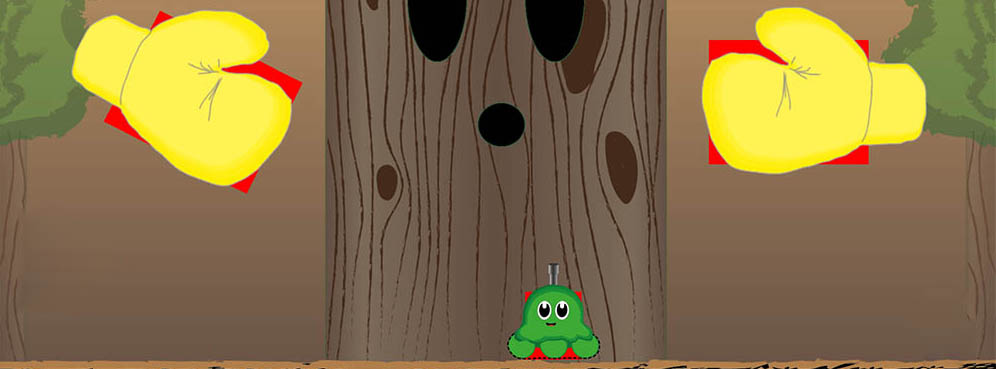
\includegraphics[width=\textwidth - 50pt]{resources/CollisionLayer_BossKampf.jpg}
  \caption{CollisionLayer Debug im Boss Kampf}
  \label{fig:collision_debug_boss} 
\end{figure}

Wenn man genau hinsieht erkennt man, dass auch Münzen über eine Kollision verfügen. Tödliche Objekte in der Karte (bsp. Dornen) jedoch nicht.

\begin{figure}[H]
  \centering
  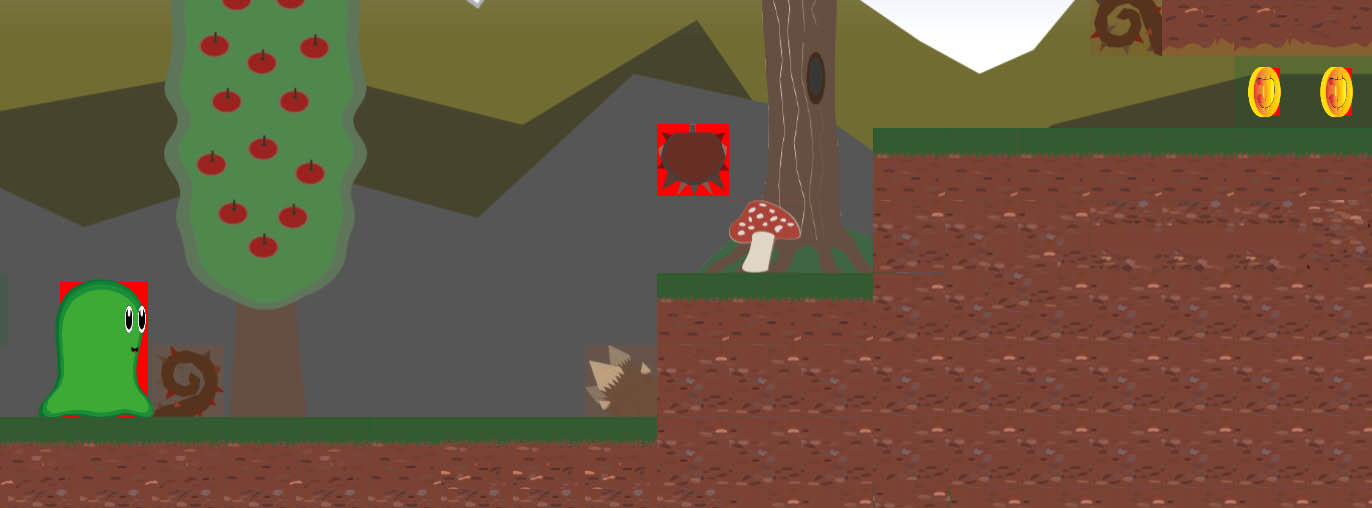
\includegraphics[width=\textwidth - 50pt]{resources/CollisionLayer_Level}
  \caption{CollisionLayer Debug im Level}
  \label{fig:collision_debug_level} 
\end{figure}


\subsection{Listener registrieren}

Die Klasse verfügt über eine Funktion \textbf{setCollisionListener(CollisionLayer*)} die ein anderes Collision Layer als Parameter erwartet. Dabei wird das übergebene Objekt in einer internen Variable gespeichert und in der \textbf{update()} Methode kontinuierlich auf Kollision überprüft.

\subsection{Gegenseite Collision Notification}

Sobald eine Kollision festgestellt wird, werden beide Objekte darüber informiert. Die Methode \textbf{hitByCollision(CollisionLayer*)} ist in der \josieclass{CollisionLayer} Klasse nicht implementiert und muss von den einzelnen Subklassen durch Logik ergänzt werden.

So wird bei einem \josieclass{StageHazard} - im Falle einer Collision mit dem Spieler - das tödliche Objekt wieder auf Anfang positioniert.

\begin{lstlisting}[label=lst:hit_by_collision,
				   language=C++,
				   firstnumber=32,
				   caption=Collision Notification ( StageHazard.cpp )]
void StageHazard::hitByCollision(CollisionLayer* other)
{
	if (other->collisionType == CollisionLayerTypeLevelPlayer) {
		this->fallDown();
	}
}
\end{lstlisting}
